% Copyright 2016-2023 - Julien TREBOSC, Bas van Meerten and Wouter Franssen
%
%This file is part of ssNake.
%
%ssNake is free software: you can redistribute it and/or modify
%it under the terms of the GNU General Public License as published by
%the Free Software Foundation, either version 3 of the License, or
%(at your option) any later version.
%
%ssNake is distributed in the hope that it will be useful,
%but WITHOUT ANY WARRANTY; without even the implied warranty of
%MERCHANTABILITY or FITNESS FOR A PARTICULAR PURPOSE.  See the
%GNU General Public License for more details.
%
%You should have received a copy of the GNU General Public License
%along with ssNake. If not, see <http://www.gnu.org/licenses/>.

\documentclass[11pt,a4paper]{article}
% Copyright 2016 - 2017 Bas van Meerten and Wouter Franssen
%
%This file is part of ssNake.
%
%ssNake is free software: you can redistribute it and/or modify
%it under the terms of the GNU General Public License as published by
%the Free Software Foundation, either version 3 of the License, or
%(at your option) any later version.
%
%ssNake is distributed in the hope that it will be useful,
%but WITHOUT ANY WARRANTY; without even the implied warranty of
%MERCHANTABILITY or FITNESS FOR A PARTICULAR PURPOSE.  See the
%GNU General Public License for more details.
%
%You should have received a copy of the GNU General Public License
%along with ssNake. If not, see <http://www.gnu.org/licenses/>.

\usepackage[british]{babel}
\usepackage{graphicx,booktabs,listings,amsmath,pgfplots,pgfplotstable}
\usepackage[small,bf,nooneline]{caption}
\usepackage{subcaption}
\usepackage[sort&compress,numbers]{natbib}
\usepackage{tikz}
\usepackage{mathtools}
\usepackage[nottoc]{tocbibind}%adds bibliography to table of contents.
\graphicspath{{./images/}}
%\setlength{\textwidth}{453pt} %597 pt is the a4 paperwidth. Minus 2 in margin. 72 pt = 1 in
%\setlength{\hoffset}{-\oddsidemargin}
%\setlength{\voffset}{-30pt} %
%\setlength{\textheight}{651 pt} %a4 height 845 pt minus 2* total headheight. In this case 2*88pt
%% examine margines via the layout package. Use command \layout{} in document to draw a picture.
%\setlength{\parindent}{0.5 cm}
%\setlength{\parskip}{0 cm}
\usepackage[left=82pt,right=82pt,top=95pt,bottom=95pt,footnotesep=0.5cm]{geometry}
%\setlength{\headheight}{14pt}

%define colours--------------------
%dark
\usepackage{xcolor}
\definecolor{MyGrayD}{RGB}{1,1,1}
\definecolor{MyRedD}{RGB}{237,45,46}
\definecolor{MyGreenD}{RGB}{0,140,71}
\definecolor{MyBlueD}{RGB}{24,89,169}
\definecolor{MyOrangeD}{RGB}{243,125,34}
\definecolor{MyPurpleD}{RGB}{102,44,145}
\definecolor{MyBrownD}{RGB}{161,29,32}
\definecolor{MyPinkD}{RGB}{179,56,147}
%normal
\definecolor{MyGray}{RGB}{114,114,114}
\definecolor{MyRed}{RGB}{241,89,95}
\definecolor{MyGreen}{RGB}{121,195,106}
\definecolor{MyBlue}{RGB}{89,154,211}
\definecolor{MyOrange}{RGB}{249,166,90}
\definecolor{MyPurple}{RGB}{158,102,171}
\definecolor{MyBrown}{RGB}{205,112,88}
\definecolor{MyPink}{RGB}{215,127,179}
%light
\definecolor{MyGrayL}{RGB}{204,204,204}
\definecolor{MyRedL}{RGB}{242,174,172}
\definecolor{MyGreenL}{RGB}{216,228,170}
\definecolor{MyBlueL}{RGB}{184,210,235}
\definecolor{MyOrangeL}{RGB}{242,209,176}
\definecolor{MyPurpleL}{RGB}{212,178,211}
\definecolor{MyBrownL}{RGB}{221,184,169}
\definecolor{MyPinkL}{RGB}{235,191,217}
%----------------------------------

%Figure ref with hyperref
\newcommand{\fref}[1]{\hyperref[#1]{Figure \ref*{#1}}}
\newcommand{\sref}[1]{\hyperref[#1]{Section \ref*{#1}}}
\newcommand{\tref}[1]{\hyperref[#1]{Table \ref*{#1}}}

%Makes a new command for figures with input values: filename, width(times linewidth),
% caption and label.
\newcommand{\onefigure}[4]{
\setlength{\captionwidth}{#2\linewidth}
\begin{figure}
\includegraphics[width=#2\linewidth]{#1}
\centering
\parbox{\linewidth}{\caption{#3}
\label{#4}}
\end{figure}
}

%Makes a new command for tikz figures with input values: tikz commands, 
% caption and label.
\newcommand{\onetikz}[3]{
\settowidth{\captionwidth}{#1}
\ifthenelse{\lengthtest{\captionwidth<0.7\linewidth}}{\setlength{\captionwidth}{0.7\linewidth}}{}

\begin{figure}
\centering
#1
\centering
\parbox{\linewidth}{\caption{#2}
\label{#3}}
\end{figure}
}

%Makes a new command for two figures next to each other with input values: filename1, caption1, label1,filename2, caption2 and label2. Figure width is set to 0.47\linewidth and the space between the figures is filled with \hfill so the sides of the figures align with to edge of the line.
\newcommand{\twofigure}[6]{
\setlength{\captionwidth}{\linewidth}
\begin{figure*}[ht!]
\begin{minipage}[t]{0.47\linewidth}
\includegraphics[width=\linewidth]{#1}
\centering
\caption{#2}
\label{#3}
\end{minipage}
\hfill
\begin{minipage}[t]{0.47\linewidth}
\centering
\includegraphics[width= \linewidth]{#4}
\centering
\caption{#5}
\label{#6}
\end{minipage}
\end{figure*}
}


%Makes a new command for a table with caption witdh equal to the total table width. Input: tabular, caption and label. Example:
%\onetable{
%\begin{tabular}{ccc}
%a&b&c\\
%\hline
%1&1&1\\
%1&1&1\\
%1&1&1\\
%\end{tabular}
%{The caption.}
%{tab:table1}
%}
\newcommand{\onetable}[3]{
\settowidth{\captionwidth}{#1}
\ifthenelse{\lengthtest{\captionwidth<0.7\linewidth}}{\setlength{\captionwidth}{0.7\linewidth}}{}
\begin{table}
\caption{#2}
\vspace{-0.24cm} %Puts caption close to toprule
\label{#3}
\centering
#1
\end{table}
}

%Makes a long table with captionwidth equal to tablewidth. It takes the following arguments:
%1: Column specifier (e.g. cccc)
%2: Caption
%3: Label
%4: First head (i.e. first row of regular table)
%5: Head of consecutive pages
%6: Foot of pagebreak
%7: Lastfoot (e.g. \midrule)
%8: Body of table
\newcommand{\onelongtable}[8]{
\begin{center}
\settowidth{\captionwidth}{
\begin{tabular}{#1}
#4
#8
\end{tabular}} % This ends the captionwidth part. Next comes the real table.

\begin{longtable}{#1}
\caption{#2}\\
\vspace{-0.74cm} %Puts caption close to toprule
\label{#3}\\

#4
\endfirsthead

#5
\endhead

#6
\endfoot

#7
\endlastfoot

#8
\end{longtable}
\end{center}}




%1:pgfplots code
%2:width
%3:caption
%4:label
\newcommand{\pgfplotsfigure}[4]{
\pgfplotsset{width=#2\linewidth}
\setlength{\captionwidth}{#2\linewidth}
\begin{figure}[t]
\centering
#1
\centering
\parbox{\linewidth}{\caption{#3}
\label{#4}}
\end{figure}
}


\usepackage[bitstream-charter]{mathdesign}
\usepackage[T1]{fontenc}
\usepackage[protrusion=true,expansion,tracking=true]{microtype}
\pgfplotsset{compat=1.7,/pgf/number format/1000 sep={}, axis lines*=left,axis line style={gray},every outer x axis line/.append style={-stealth'},every outer y axis line/.append style={-stealth'},tick label style={font=\small},label style={font=\small},legend style={font=\footnotesize}}
\usepackage{colortbl}
\usetikzlibrary{calc}

%Set section font
\usepackage{sectsty}
\allsectionsfont{\color{black!70}\fontfamily{SourceSansPro-LF}\selectfont}
%--------------------


%Set toc fonts
\usepackage{tocloft}
%\renewcommand\cftchapfont{\fontfamily{SourceSansPro-LF}\bfseries}
\renewcommand\cfttoctitlefont{\color{black!70}\Huge\fontfamily{SourceSansPro-LF}\bfseries}
\renewcommand\cftsecfont{\fontfamily{SourceSansPro-LF}\selectfont}
%\renewcommand\cftchappagefont{\fontfamily{SourceSansPro-LF}\bfseries}
\renewcommand\cftsecpagefont{\fontfamily{SourceSansPro-LF}\selectfont}
\renewcommand\cftsubsecfont{\fontfamily{SourceSansPro-LF}\selectfont}
\renewcommand\cftsubsecpagefont{\fontfamily{SourceSansPro-LF}\selectfont}
%--------------------

%Define header/foot
%\usepackage{fancyhdr}
%\pagestyle{fancy}
%\fancyhead[LE,RO]{\fontfamily{SourceSansPro-LF}\selectfont \thepage}
%\fancyhead[LO,RE]{\fontfamily{SourceSansPro-LF}\selectfont \leftmark}
%\fancyfoot[C]{}
%--------------------

%remove page number from first chapter page
%\makeatletter
%\let\ps@plain\ps@empty
%\makeatother
%----------------------

\usepackage[hidelinks,colorlinks,allcolors=black, pdftitle={Advanced MQMAS processing in ssNake},pdfauthor={Julien TRÉBOSC}]{hyperref}

\interfootnotelinepenalty=10000 %prevents splitting of footnote over multiple pages
\linespread{1.2}

\title{\color{black}\fontfamily{SourceSansPro-LF}\bfseries Advanced MQMAS processing in ssNake}
\author{}
\date{\color{black}\fontfamily{SourceSansPro-LF}\bfseries \today}


\begin{document}
%\newgeometry{left=72pt,right=72pt,top=95pt,bottom=95pt,footnotesep=0.5cm}
\microtypesetup{protrusion=true} % enables protrusion

\maketitle

%%%%%%%%%%%%%%%%%%%%%%%%%%%%%%%%%%%%%%%%%%%%%%%%%%%%%%%%%%%%%%%%%%%%%%%%%%%%%%%%%%%%%%%%%%%%%%%%%%%%
\section{Introduction}
This tutorial will make a review of MQMAS experiment principles and will present several ways to process and fit 
Multiple Quantum Magic Angle spinning (MQMAS) NMR data using ssNake.
The tutorial delivered with the ssNake program is considered as prior knowledge and having done MQMAS tutorial is advized.
If you have not yet studied this, please do so before continuing with these examples.

This tutorial is assuming ssNake version 1.5 to be used. There is a change on sign of shearing and scaling with respect to 
previous versions depending on spin I and MQ level. ssNake v1.5 calculations for shearing and scale assume an evolution on 
$-pQ$ ($p=$3, 5, 7 or 9 for MQMAS and $p= 1 or 2$ for STMAS and DQ-STMAS. While previous versions assume a coherence pathway 
such that quadrupolar echo is shifting towards positive $t_2$ time.

%%%%%%%%%%%%%%%%%%%%%%%%%%%%%%%%%%%%%%%%%%%%%%%%%%%%%%%%%%%%%%%%%%%%%%%%%%%%%%%%%%%%%%%%%%%%%%%%%%%%
\section{MQMAS principles}
MQMAS is a 2D experiment for half-integer quadrupolar nuclei which is used to obtain isotropic information from nuclei 
broadened by the second order quadrupole interaction. This allows the separation of multiple overlapping quadrupolar 
sites on the basis of their `isotropic' value (which is a combination of the isotropic chemical shift, and the isotropic 
quadrupolar shift, which is also called the quadrupolar induced shift). 

The experiment can be quite difficult to process.
Not because of the complication of the steps involved, but due to the large number of different MQMAS experiments and the various ways to process these.
This advanced tutorial will give several examples of MQMAS processing in various cases and give hints on parameters that must be
considered to run processing in the proper way.
Moreover, it will explain how to simulate different kind of processing.

The principle of MQMAS is to correlate $-pQ$ coherence ($p=3$, 5, 7 or 9) during $t_1$ evolution with the observable $-1Q$ 
coherence. The total signal phase evolution during $t_1$ and $t_2$ is 
$$\omega_Q(-pQ) \cdot t_1 + \omega_Q(-1Q) \cdot t_2$$
for quadrupolar interaction and
$$\omega_{CS}(-pQ) \cdot t_1 + \omega_{CS}(-pQ) \cdot t_2$$
for chemical shift interaction.

The dephasing can cancel at a point in $t_2$ evolution when $t_2 = - {\omega(-pQ) \over \omega(-pQ)} t_1$.
The ratio of dephasing occuring during $-pQ$ and $-1Q$ is
$$R={\omega_Q(-pQ) \over \omega_Q(-1Q)}$$
for the second order quadrupolar interaction and
$${\omega_{CS}(-pQ) \over \omega_{CS}(-1Q)} = p $$
for the chemical shift interaction.

The reason for MQMAS to be working is that ratios R and p are independant of $C_Q$/$\eta_Q$ and chemical shift 
amplitudes respectively, and these ratio are different ($R \neq p$) which allows to separate their contributions along 
different axes.
Depending on p and spin S, the ratio R of quadrupolar dephasing can be positive or negative. For chemical shift the ratio is $+p$.
A negative ratio means that dephasing in $t_1$ and $t_2$ are canceling leading to the formation of an echo at positive time 
($t_2 = - R \cdot t_1$).
A positive ratio means that dephasings are cumulative in $t_1$ (evolution on $-pQ$) and $t_2$ (evolution on $-1Q$). 
The echo is shifting to negative $t_2$. Note that a positive R will result in a spectrum correlation with 
slope $F_1=R\cdot F_2$, but a quadrupolar echo that shifts with $t_2 = -R \cdot t_1$.

Depending on the dominating interaction one can observe the formation of an echo at position $t_2 = -R \cdot t_1$ if 
the quadrupolar interaction is strong or at $t_2 = -3 \cdot t_1$ if chemical shift distribution is dominating.

Z-Filter MQMAS is acquired in hyper-complex mode (for example State): echo and anti-echo are recorded simultaneously so a signal
is always observed at positive $t_2$. The way quadrature is implemented (within the pulse sequence and hardware) will select 
the $\pm pQ$ pathway (more often the expected $-pQ$).
A full echo MQMAS only selects one pathway. It can be $\pm pQ$ depending on the pulse sequence implementation and on the 
requirement to have signal in positive acquisition time ($t_2$). Indeed very often the pulse sequence will select the pathway
for which an echo shifts towards increasing $t_2$ times ($R < 0$).
If $+pQ$ is selected by the pulse sequence, then one will need to perform a Complex conjugate operation on D1 time domain, 
or a flip Left/Right operation on D1 frequency domain to flip the spectrum (indeed $\omega(pQ) = -\omega(-pQ)$).

Therefore, apodization should be done along $-R$ axis (or $\pm$R axes for Z-Filter MQMAS when echo and anti-echo are selected).
In some experiments the dominating interaction is chemical shift distribution. In that case, the echo is mostly appearing 
at $t_2 = -p \cdot  t_1$. Then the slope for shifting should be $\pm$p. Eventualy one should look at the FID to determine the best
apodization and slope.


Shearing process aligns the correlation peaks horizontally instead of along the R slope by rolling each column (in D1 dimension). 
Shearing should always be done relative to the carrier frequency to get proper scale (the column at the carrier 
in D2 remains unchanged). In time domain shearing is equivalent to make the quadrupolar echo be positioned
at $t_2=0$ (time when second order quadrupolar dephasings are canceled). 

Once shearing is done, a universal scale can be designed that will make the peaks appear at the same position (in ppm)
whatever p is used (3QMAS, 5QMAS, or even STMAS). There are two way to achieve such scale:
\begin{itemize}
  \item Scale the spectral window (SW).
  \item Scale the carrier and reference frequencies used to calculate ppm scale).
\end{itemize}

When using SW scaling, the spinning sidebands will appear at scaled spinning speed in kHz. When using carrier and 
reference scaling, the spinning sideband separation remains at the spinning speed in kHz, however the Chemical Shift axis 
slope is scaled (due to shearing operation) and is 1 only when both axis are in ppm unit.

\subsection{Split-t1 experiments}
Split-t1 MQMAS experiments are designed to refocus the second order quadrupolar anisotropy at a fix time in D2.
This corresponds to applying a shearing processing operation. It is usually done by defining a delay $\tau$, on $\pm 1Q$ quantum
level, which duration depends on t1 (pQ coherence evolution) such that $\tau = R \cdot t_1$ before the acquisition during $t_2$.

Therefore, one just need to deal with such experiment just the same as a pQMAS experiment. The experiment does not need be sheared, 
and should be scaled as pQMAS experiment with $t_1$ evolution defined as evolution time on $pQ$. 

%%%%%%%%%%%%%%%%%%%%%%%%%%%%%%%%%%%%%%%%%%%%%%%%%%%%%%%%%%%%%%%%%%%%%%%%%%%%%%%%%%%%%%%%%%%%%%%%%%%%
\section{ssNake tools for MQMAS processing}
Note that current ssNake tools assume that the quadrupolar echo is shifting towards 
positive $t_2$ time. For example, for spin 5/2 3QMAS, it will use a ratio $R=19/12$ corresponding to 
$R = {\omega_Q(+3Q) \over \omega_Q(-1Q)}$ that is evolution on $+3Q$ during $t_1$. It will apply the corresponding 
ratio for shearing. Since in that case the spectrum in D1 is reversed, the Scale SW tool will propose to use
a negative factor (-12/17) that will reverse the D1 axis (instead of the data as when using Flip L/R tool or using 
complex conjugate in time domain before FT). 

Fitting of MQMAS will also
The simulation procedure calculate the frequency of $-pQ$ and $-1Q$ for each crystallite. The `Auto' button calculates the 
the shear and Scale SW parameters adequately. 

\section{Data}
In this tutorial we will use several datasets:
\begin{itemize}
\item a Z-filter 3QMAS of 5/2 spin nucleus (${}^{27}$Al).
\item an unconventional split-t1 full echo 3QMAS of 3/2 spin nucleus (${}^{35}$Cl).
\item a Z-filter STMAS recorded with NUS of 3/2 spin nucleus (${}^{87}$Rb).
\end{itemize}


\section{Z-Filter MQMAS processing}
First, we will look into the processing of MQMAS data recorded using a Z-Filter experiment (also called three pulse MQMAS).
Note that data recorded with a regular two pulse MQMAS (the standard MQMAS experiment) can be processed in the same way.

Open the `3QMAS-Z' dataset. This is a ${}^{27}$Al 3QMAS experiment of AlPO VPI-5 mesoporous sample. It has been recorded 
in States-TPPI mode on a 18.8~T spectrometer at 20~kHz MAS rate.

Be careful that some information in the dataset may be wrong or unexpected. Especially the carrier and reference frequencies
in dimension D1 may be already scaled (if xfshear has been applied under Topspin) or even correspond to a wrong nucleus. 
In the worst case, the SW could be wrong. This could happen if actual $t_1$ evolution increment (on Bruker this would often 
be parameter IN0) does not correspond to declared spectral window (parameter SW\_h in Bruker).

Processing of the data is performed in the following steps:
\begin{itemize}
  \item Remove digital filter.
  \item Set the view to D1 (sideframe, radiobutton).
  \item Convert the hypercomplex data via Transforms  $\longrightarrow$ Hypercomplex  $\longrightarrow$
   selecting `States-TPPI'.
  \item Set the view back to D2 (sideframe, radiobutton).
  \item Apodize in D2 using a gaussian apodization (50~Hz), with shifting (select `Spin 5/2 3QMAS' which enter a Value or 19/12).
\end{itemize}

Note the shifting option. We chose to shift apodization along the quadrupolar echo slope. But in some spectra, chemical shift 
distribution could be dominant and a slope of 3 would be better. One can also choose a compromise that is a slope in between
the two.

The FID should now look like this:
\begin{center}
%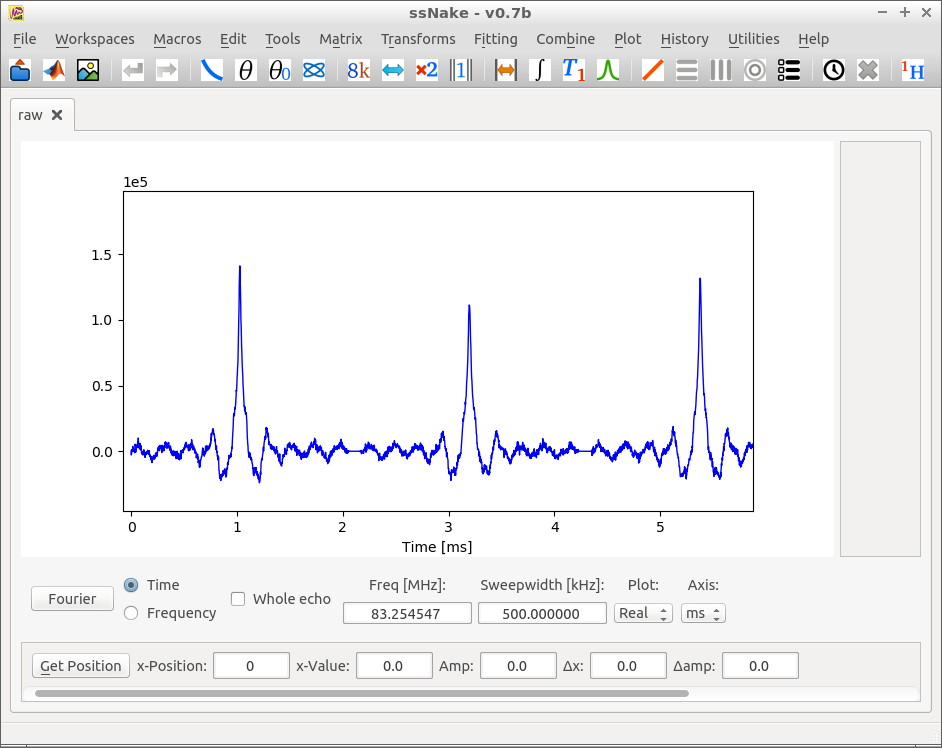
\includegraphics[width=0.8\linewidth]{Figs/Fig1.png}
\end{center}

\begin{itemize}
  \item Zero-fill (Matrix $\longrightarrow$  Sizing) 2048 points. (actual FID will be truncated).
  \item Fourier Transform D2, and phase the first slice.
  \item Set the view to D1 (sideframe, radiobutton).
  \item Processing of the indirect dimension D1 (zerofill, Fourier, apodize, phase).
\end{itemize}

At that point we have several options for processing:
\begin{itemize}
  \item whether to shear the spectrum.
  \item whether to scale the spectral width or the carrier and reference frequencies in the indirect dimension.
\end{itemize}

\subsection{3Q-1Q representation}
First we can choose to represent the spectrum in 3Q-1Q scale. To do that we need to adjust the reference frequency to $3 \cdot Ref - 2 \cdot Car$
where Ref is D2 dimension reference frequency and Car is the carrier frequency in D2 (and D1). Indeed this will ensure that the center 
of the spectrum will correspond to ppm coordinates $(F1, F2)= (p, 3p)$.
First we need to ensure that D1 Carrier and Reference frequencies in D1 correspond to D2. This may not be necessary but as said before
they may not be correct.
Go to menu `Tools' $\longrightarrow$ `Reference' $\longrightarrow$ `Set Reference'. Give name `D2' and validate.
Copy (crtl-C) the carrier frequency shown in D2 dimension. 
Select dimension D1
Paste the Carrier Frequency from D2.
Go to menu `Tools' $\longrightarrow$ `Reference' $\longrightarrow$ `Apply'. Select `D2'.
Go to menu `Tools' $\longrightarrow$ `Reference' $\longrightarrow$ `Set Reference', then apply the operation $3 Ref - 2 Car$ for 
the reference frequency (There you can also `Paste' the Carrier frequency that was copied above to write the equation).

This results in the following spectrum:
\begin{center}
%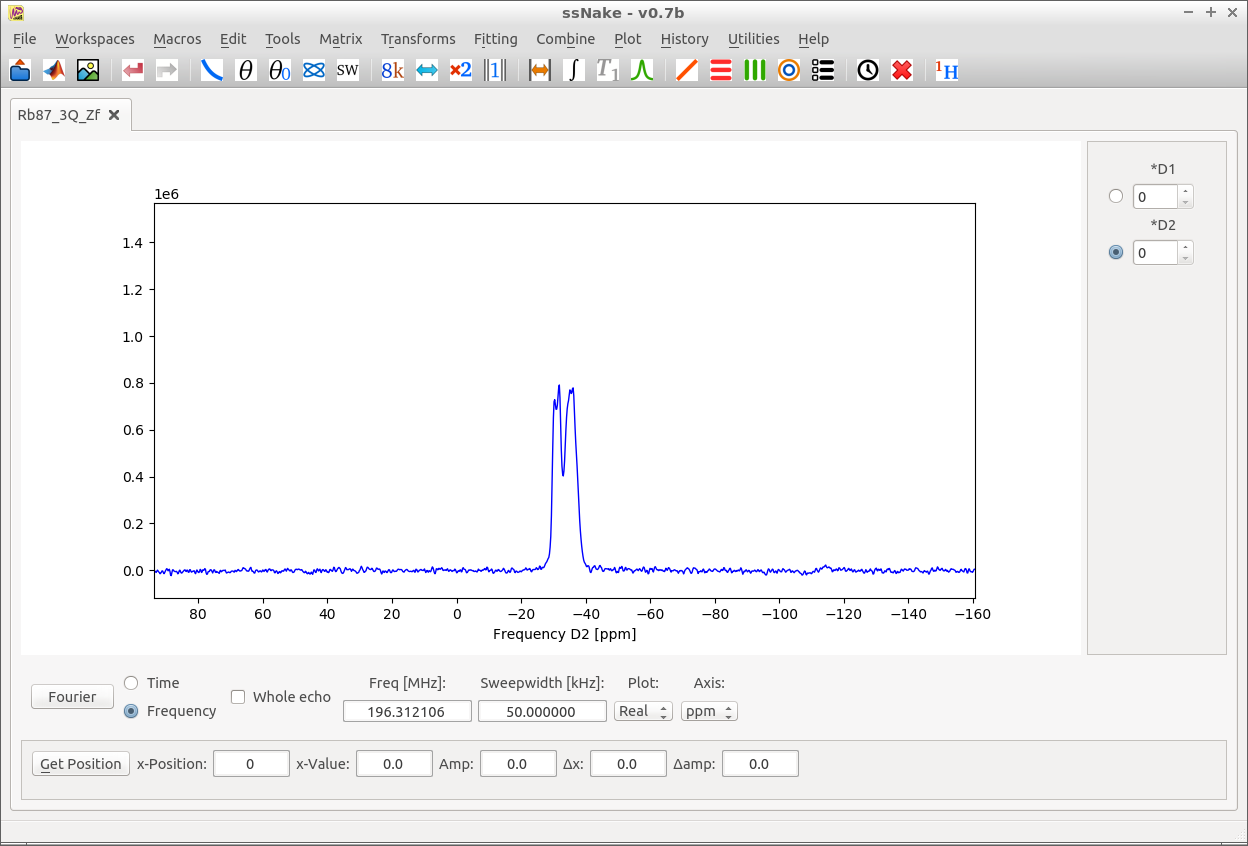
\includegraphics[width=0.8\linewidth]{Figs/Fig2.png}
\end{center}

One can fit such spectrum with MQMAS model. There are 3 sites with main parameters summarized in table \ref{table:AlPO_vpi5_sites}.

\begin{center}\label{table:AlPO_vpi5_sites}
  \begin{tabular}{c|c c c} 
	 \toprule
	 Site & $\delta_\text{iso}$ [ppm]& $C_\text{Q}$ [MHz] & $\eta_\text{Q}$ \\
	 \midrule
 1 & -10.10      &   3.448     &          0.8992       \\
 2 &  41.74      &   1.274     &          0.4267       \\
 3 &  43.69      &   2.292     &          0.8697       \\
	\bottomrule
  \end{tabular}
\end{center}

Now, we should process the indirect dimension (D1):
\begin{itemize}
	\item Switch to D1 (sideframe, radiobutton), and select data point 614 in D2.
	\item Perform a complex conjugate (Tools $\longrightarrow$ Complex Conjugate)\footnote{The Varian data
	  we loaded has a different complex definition, so a conjugate in the indirect dimension is
	required (this depends on how the pulse sequence was programmed).}
\end{itemize}
This result in:
\begin{center}
%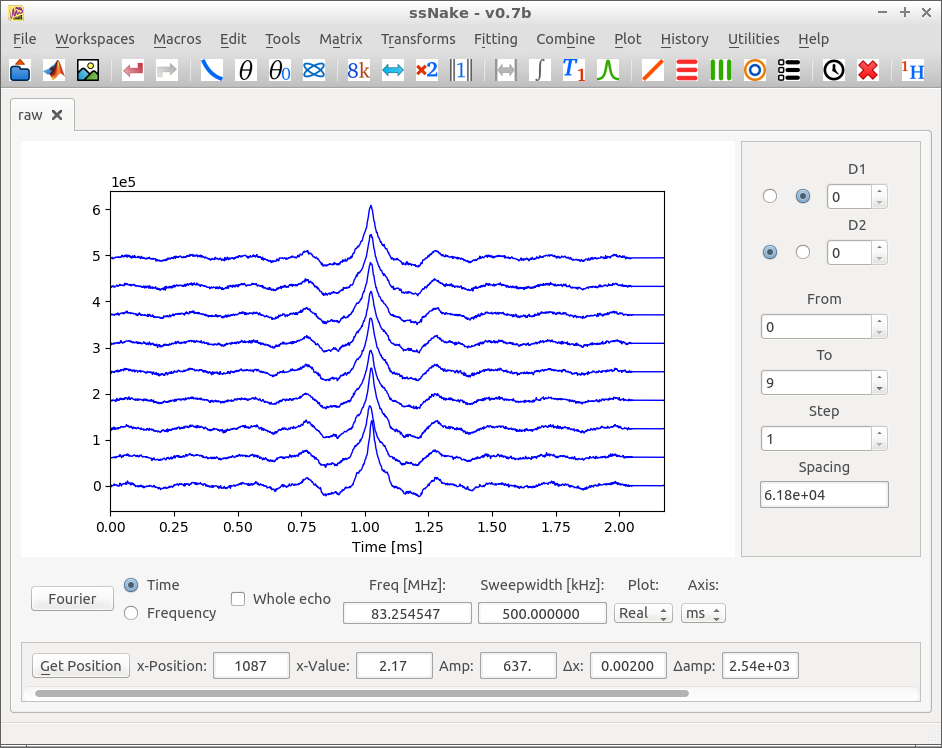
\includegraphics[width=0.8\linewidth]{Figs/Fig3.png}
\end{center}

Now we should apply some zerofilling etc.:
\begin{itemize}
	\item Set the size to 1024 points (Matrix $\longrightarrow$ Sizing)
	\item Fourier Transform
\end{itemize}
This reesults in this spectrum along D1 for this trace:
\begin{center}
%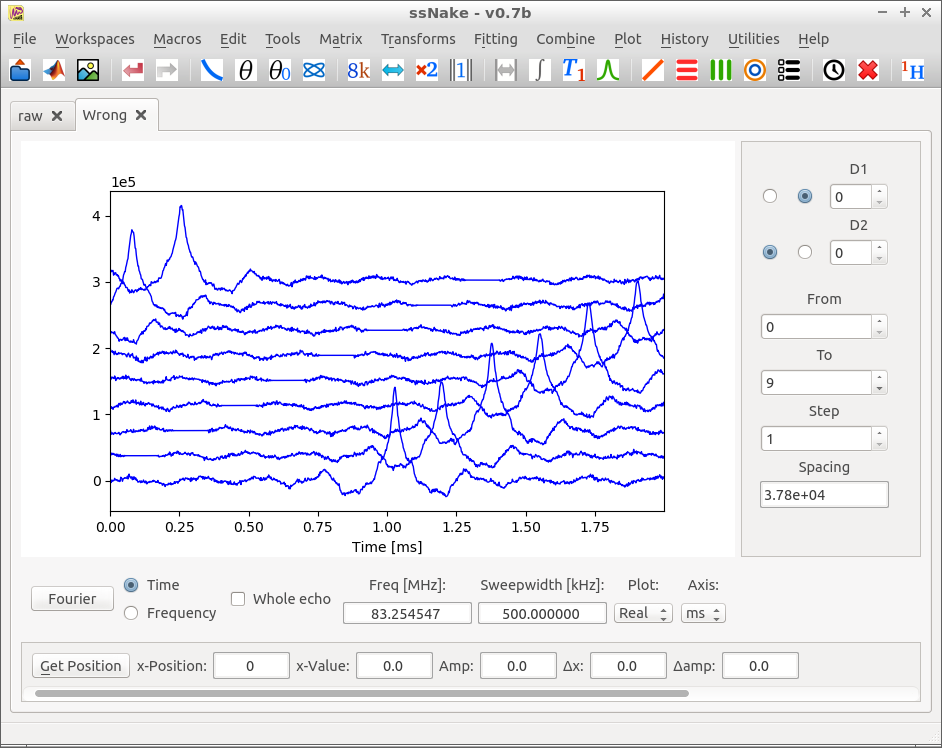
\includegraphics[width=0.8\linewidth]{Figs/Fig4.png}
\end{center}
The phase looks good, so we do not need to apply any phasing.

We have now processed both dimensions, so we can view the data as a contour plot:
\begin{itemize}
	\item Switch to D2 (sideframe, radiobutton)
	\item Change the view to a contour plot: Plot  $\longrightarrow$ Contour
\end{itemize}
We now have:
\begin{center}
%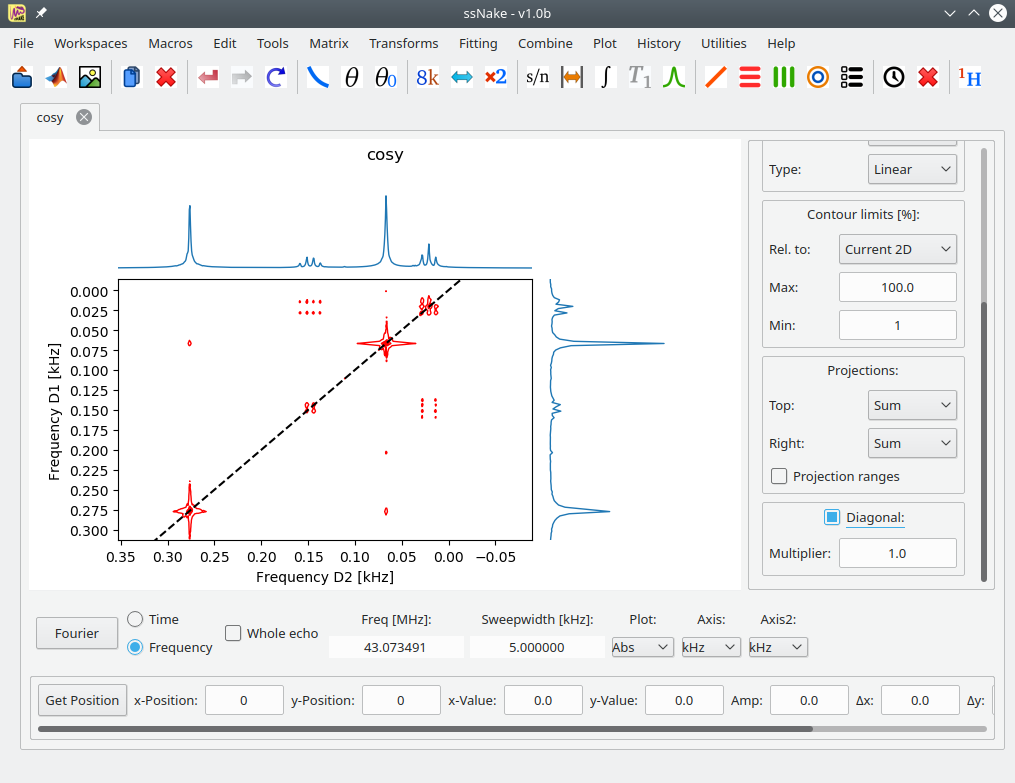
\includegraphics[width=0.8\linewidth]{Figs/Fig5.png}
\end{center}
And zoomed:
\begin{center}
%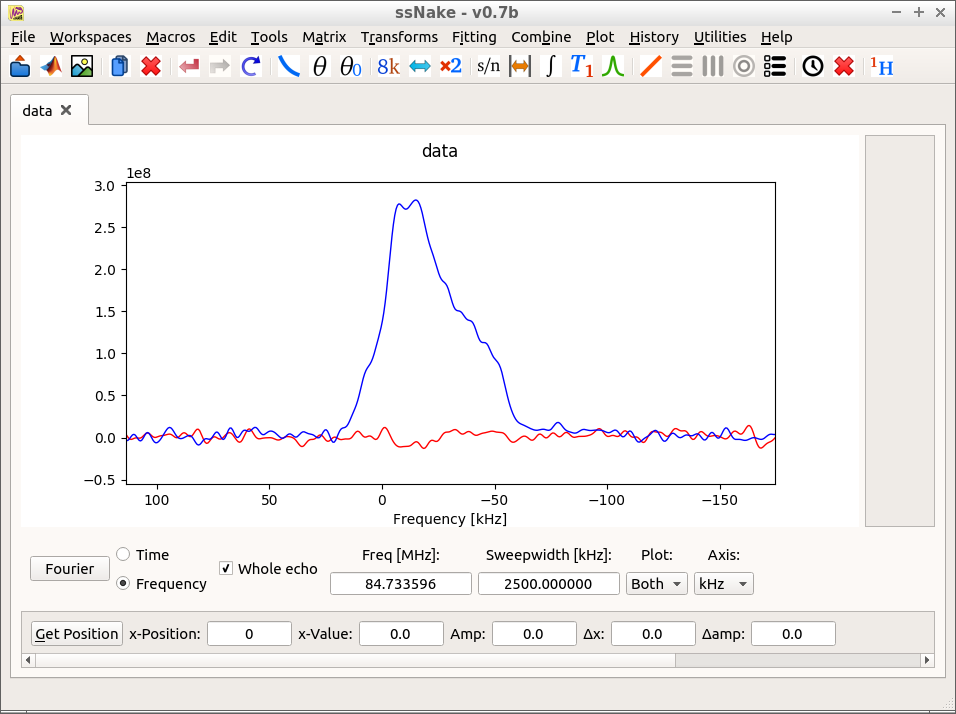
\includegraphics[width=0.8\linewidth]{Figs/Fig6.png}
\end{center}
Note that the right projection was changed to `Max' instead of the standard `Sum'.
This results in a skyline projection, which is affected less by the noise regions of the data.

As can be seen, the different powder patterns are all tilted.
This is expected for a Z-Filter MQMAS, and can be corrected by shearing the spectrum.
\begin{itemize}
	\item Shear via Matrix $\longrightarrow$ Shearing, using the `Spin 3/2, -3Q' setting, and
	  direction `1' and axis '2'
\end{itemize}
This results in (zoomed):
\begin{center}
%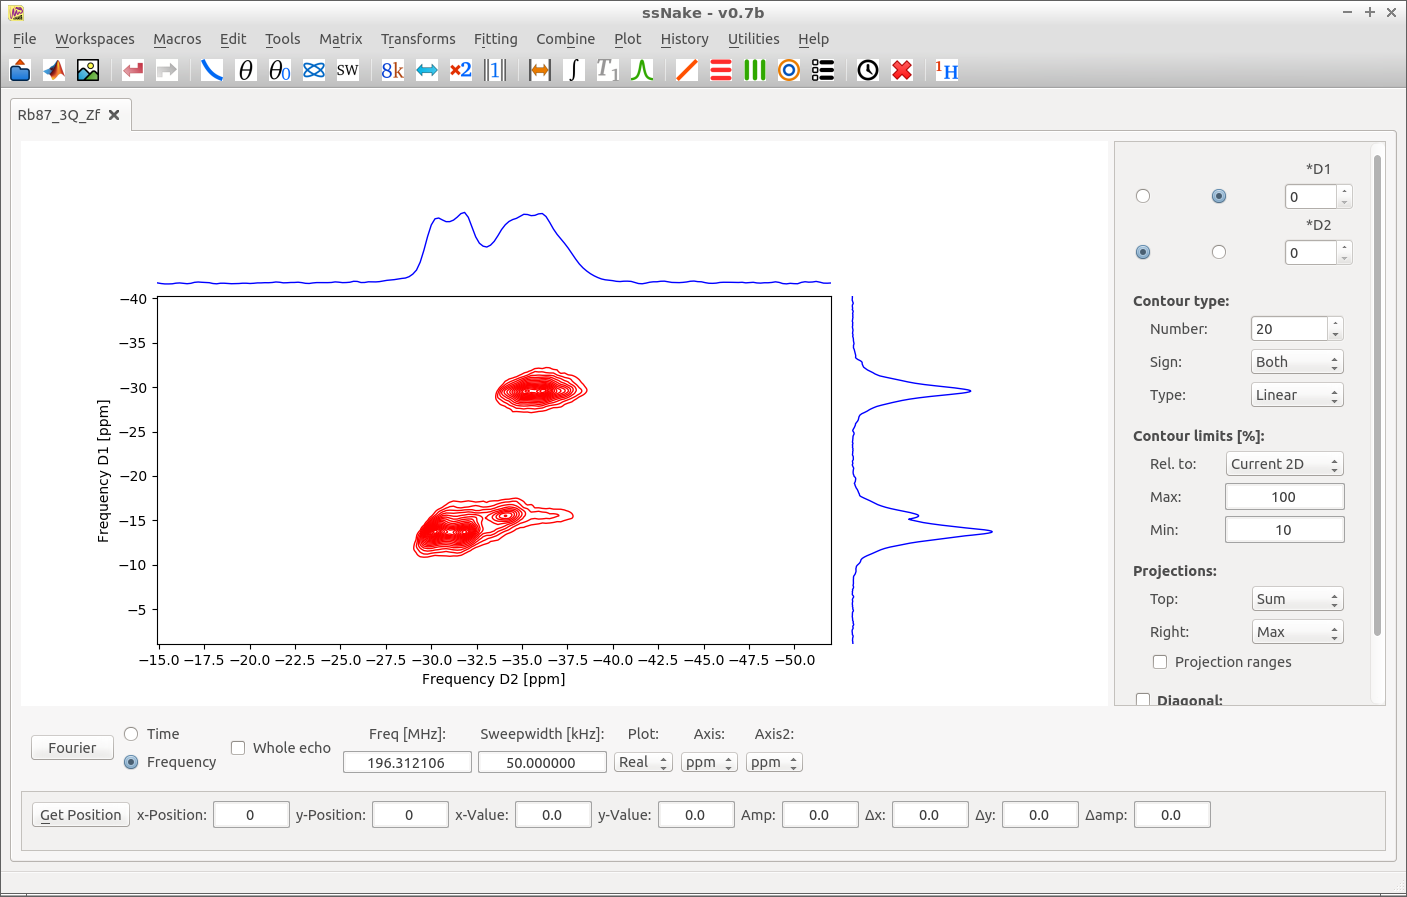
\includegraphics[width=0.8\linewidth]{Figs/Fig7.png}
\end{center}
Which is a nice spectrum! This is the final figure, we now only need to fix the axes.

By processing the spectrum in this way, we have removed the second order quadrupolar broadening from the indirect dimension.
This dimension is therefore referred to as the isotropic dimension.
The position along this axis is determined by the scaled isotropic chemical shift, and the scaled quadrupole induced shift.
However, it is more convenient to have a frequency axis which shows the unscaled isotropic chemical shift.
To accomplishing this, we must scale the spectral width by a specific value (which depends on the spin quantum number and the MQ transition of the experiment).
\begin{itemize}
	\item Switch to D1 (sideframe, click on the upper left radiobutton)
	\item Use Tools  $\longrightarrow$ Scale SW, and select `Spin 3/2, -3Q' and apply
\end{itemize}
Now, we have scaled the axis.
As a last step, we should apply the chemical shift reference.
This was determined using a rubidium nitrate solution.
Based on this the 0 ppm frequency is at: 196.3182865 MHz.
\begin{itemize}
  \item Set the reference via Tools $\longrightarrow$ Reference $\longrightarrow$ Set Reference, and
	 put `196.3182865' in the Frequency box
	\item Switch to D2 (sideframe, click on the lower left radiobutton)
	\item Set the reference in the same way
\end{itemize}
The final spectrum should now look like this (zoomed):
\begin{center}
%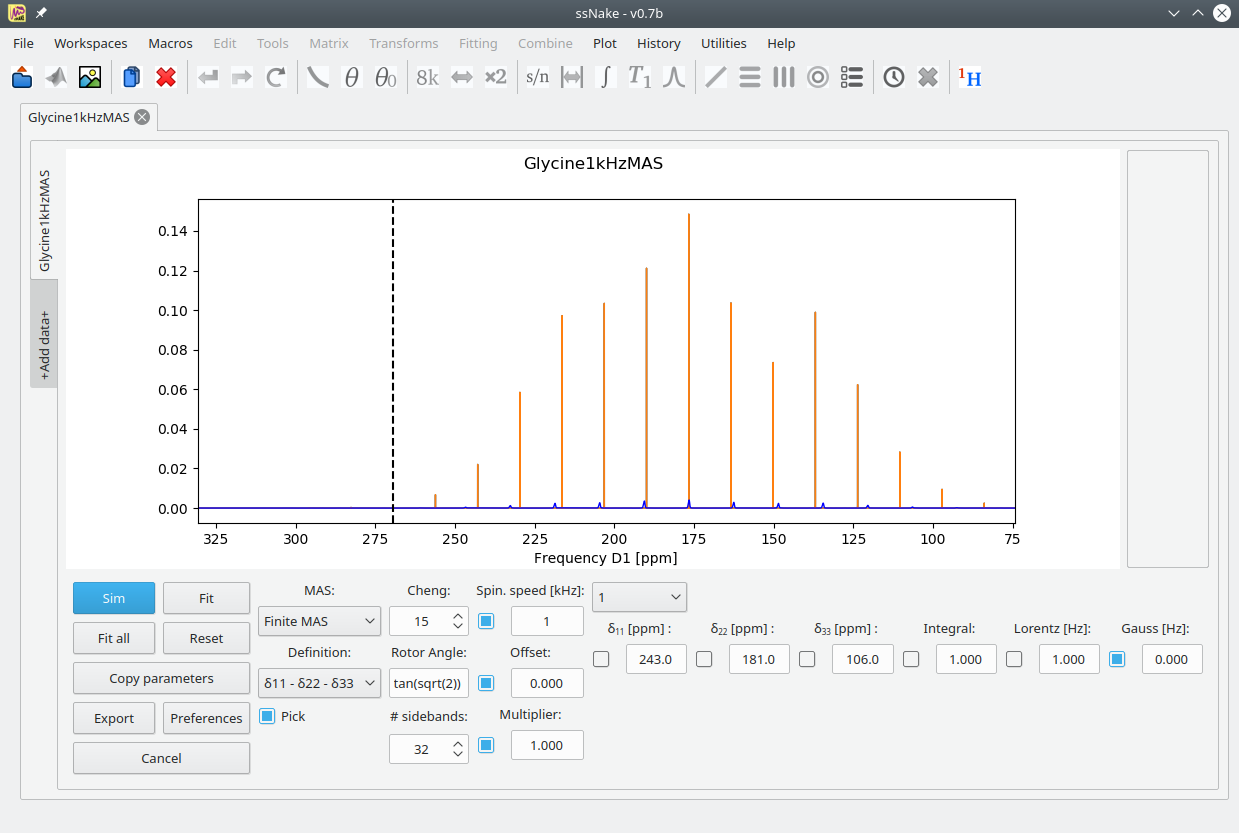
\includegraphics[width=0.8\linewidth]{Figs/Fig8.png}
\end{center}
This spectrum is also delivered with this tutorial, and named `Rb87\_3Q\_Zf\_(final\_spectrum).mat'.
Note that I extracted the relevant region before saving (to reduce size of the file).
 
Now, we can fit this spectrum.
Either by fitting a specific trace with a regular second order quadrupolar line, or by fitting the entire MQMAS spectrum.
Another alternative is to only determine the isotropic shift and the quadupolar product $P_\text{Q} = C_\text{Q}\sqrt{1+\eta^2/3}$.
For this, we must determine the Centre of Mass for each site, in both D1 and D2.
This can be done by going to the relevant trace, and using Fitting  $\longrightarrow$ Centre of Mass.
Note that in D1, the peaks are symmetric, so the highest point is the centre in this case.

\begin{center}
  \begin{tabular}{c|cc| c c}
	 \toprule
	 Site & $\delta_1$ [ppm]& $\delta_2$ [ppm]& $\delta_\text{iso}$ [ppm]& $P_\text{Q}$ [MHz]  \\
	 \midrule
	 1 & $-30.5$ & $-34.17$ & $-31.86$ & 1.89 \\
	 2& $-26.8$ &$-31.96$  &$-28.71$ & 2.24\\
	 3& $-26.3$ &$-29.76$ & $-27.58$ & 1.83 \\
	\bottomrule
  \end{tabular}
\end{center}
The last two columns have been calculated using the MQMAS Extraction utility (see the Utilities menu). 


\section{Split \textit{T}$_\text{1}$ processing}
In a split $T_\text{1}$ experiment, the additional shift of the echo is taken into account within the pulse sequence.
This leads to regular echo data, were the position of the echo in the time domain is always the same.
Due to this, the shearing is no longer required.
Also, the data is recorded in such a way that no hypercomplex processing is necessary.
The following assumes that you have read the information above (about the Z-Filter processing).

\begin{itemize}
	\item Open the Varian file Rb87\_3Q\_splitt1.fid using File $\longrightarrow$ Open
\end{itemize}
Now, we must process this data as a whole echo acquisition (see the tutorial on this).

\begin{itemize}
	\item Swap the echo at position 375 (Tools $\longrightarrow$ Swap Echo)
	\item Set the size to 4096 points (Matrix $\longrightarrow$ Sizing)
	\item Apply apodization if required (not used in this case)
	\item Fourier Transform
	\item Phase the imaginary part to zero (168.9 degrees, via Tools $\longrightarrow$ Phasing)
\end{itemize}
This should result in (zoomed):
\begin{center}
%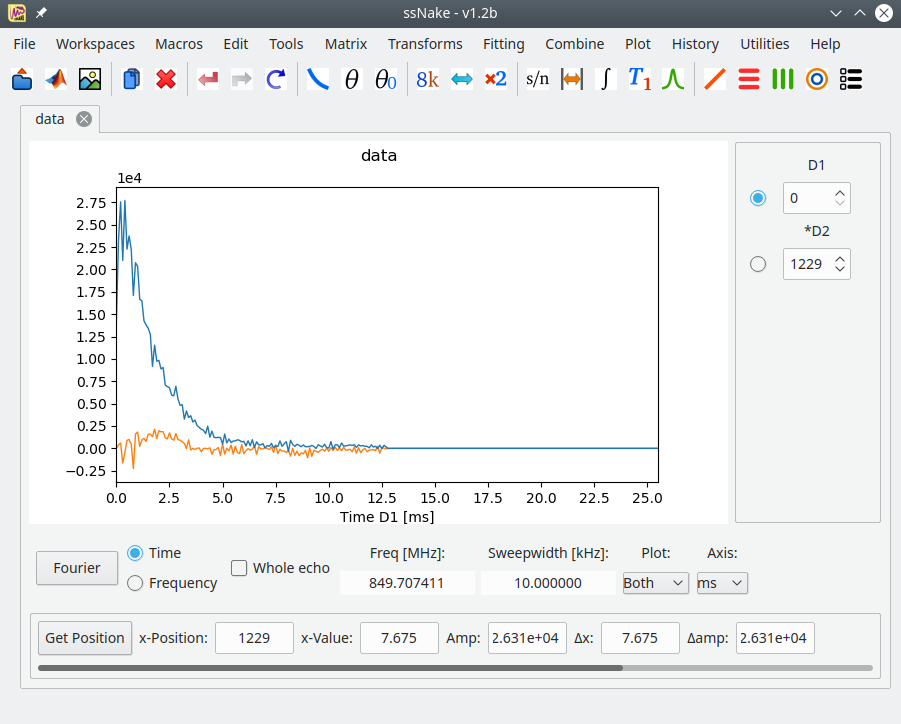
\includegraphics[width=0.8\linewidth]{Figs/Fig9.png}
\end{center}
Now we can process D1:

\begin{itemize}
	\item Switch to D1 (sideframe, radiobutton)
	\item View position 2081 along D2
	\item Tools $\longrightarrow$  Complex Conjugate
	\item Set size to 512
	\item Fourier Transform
\end{itemize}
This results in:
\begin{center}
%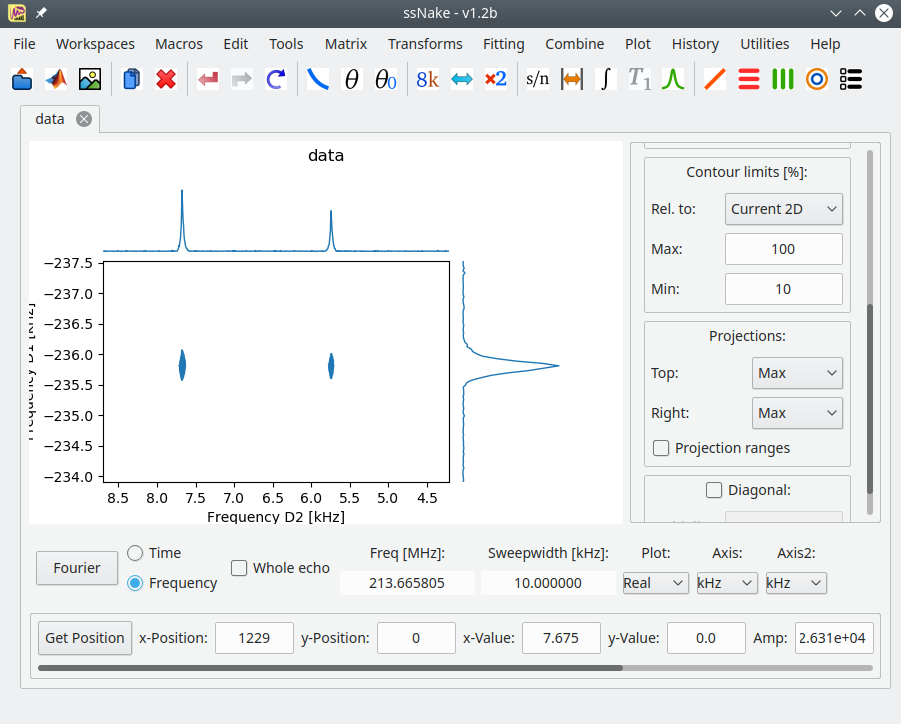
\includegraphics[width=0.8\linewidth]{Figs/Fig10.png}
\end{center}

Now, me must scale the spectral width of this dimension, as described above.
However, with this experiment something strange is going on.
According to the Varian pulse sequence used to record this data, the SW that you supply is $9/16$ times the desired spectral width.
For the processing, this means that this scaling should first be undone.

\begin{itemize}
	\item Multiply the spectral width by 16.0/9.0 (either via Tools  $\longrightarrow$ Scale SW, or
	  by typing at the SW box in the bottom frame).
	\item Multiply the SW by the MQMAS scaling value: Tools  $\longrightarrow$ Scale SW, and select `Spin 3/2, -3Q'
\end{itemize}
Now, we should reference the ppm axis in both dimension.
As before:
\begin{itemize}
  \item Set the reference via Tools $\longrightarrow$ Reference $\longrightarrow$ Set Reference, and
	 fill in `196.3182865' in the Frequency box
	\item Switch to D2 (sideframe, click on the lower left radiobutton)
	\item Set the reference in the same way
\end{itemize}
Switching to a contour plot results in (zoomed):
\begin{center}
%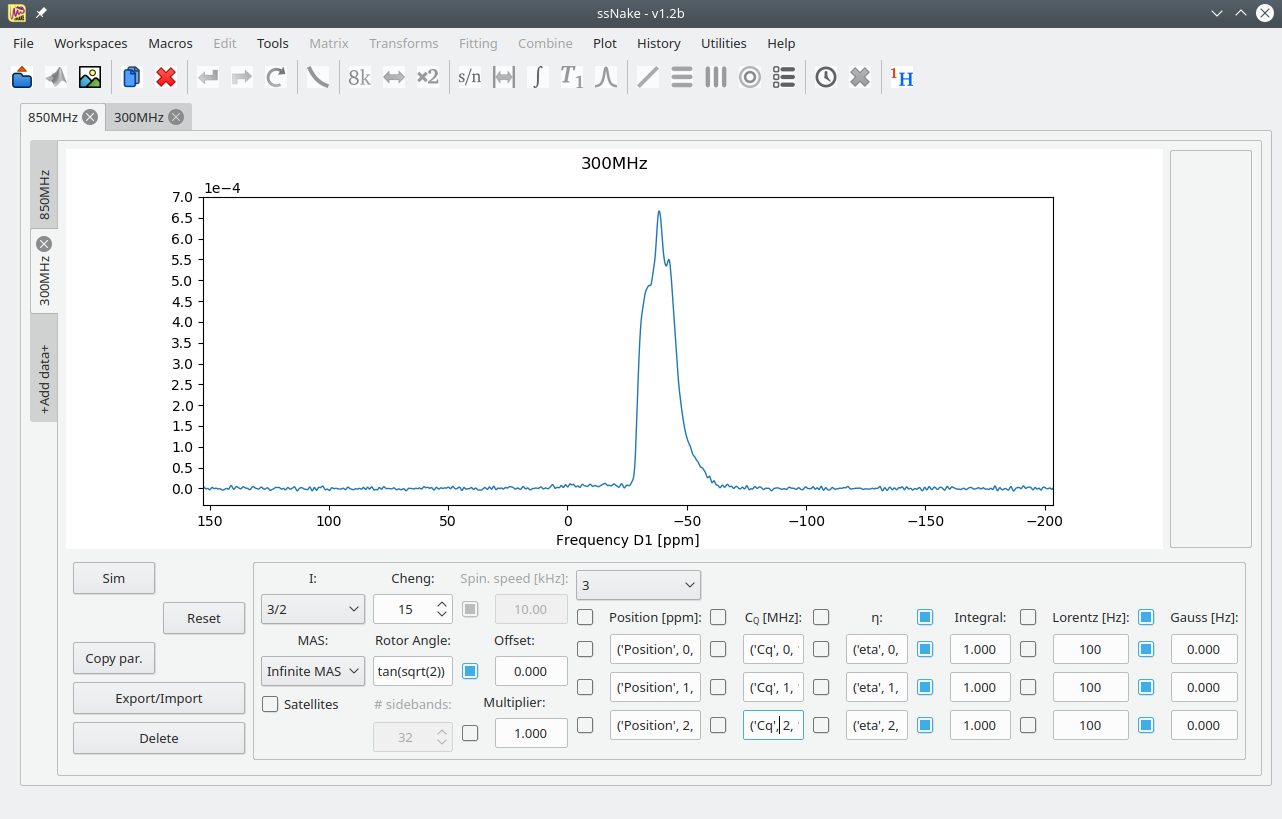
\includegraphics[width=0.8\linewidth]{Figs/Fig11.png}
\end{center}
This is equivalent to the spectrum obtained before, for the Z-Filter data.
This spectrum is also supplied together with this tutorial, and named `Rb87\_3Q\_splitt1\_(final\_spectrum).mat'.
Note that the relevant region was extracted (to reduce the size of the file).


\section{Equations}
The following Section will show some equations for the relevant shearing and scaling constants used
for MQMAS processing.\footnote{This sections is based on:
  P.\ P.\ Man, \textit{Phys.\ Rev.\ B}, \textbf{5}, 2764 (1998) and 
  T.\ Anup\~{o}ld, A.\ Reinhold, P.\ Sarv, A.\ Samoson, \textit{Solid State Nucl.\ Magn.\ Reson.},
  \textbf{13}, 87 (1998).}

These are all included in ssNake in such a way that there is no need to remember these values.
However, for the sake of completeness, they are provided here.

The following table summarises the values:
\begin{center}
\begin{tabular}[h]{c r r r r}
  \toprule
  $I$ & p$Q$ & $k$ & 1/$a$ & $z$\\
  \midrule
  3/2 & $-3Q$ & 7/9 & 9/34 & 680/27\\
  5/2 & $3Q$ & 19/12 & $-12/17$& 8500/81\\
   & $-5Q$ & 25/12 &12/85& 8500/81 \\
  7/2 & $3Q$ & 101/45 & $-45/34$& 6664/27 \\
   & $5Q$ & 11/9 & $-9/34$ & 6664/27\\
   & $-7Q$ & 161/45 & $45/476$ & 6664/27\\
  9/2 & $3Q$ & 91/36 &  $-36/17$ & 1360/3 \\
   & $5Q$ & 95/36 & $-36/85$ & 1360/3 \\
	& $7Q$ & 7/18 & $-18/117$ & 1360/3 \\
	& $-9Q$ & 31/6 & 6/85 & 1360/3 \\
  \bottomrule
\end{tabular}
\end{center}
Here, $k$ is the shearing factor, $1/a$ the scaling of the spectral width, and $z$ is a value required to determine the quadrupolar product $P_\text{Q}$ from an MQMAS spectrum (see later).
The equations are:
\begin{equation}
  k = p \frac{36I(I+1)-17p^2 - 10}{36I(I+1) - 27}
\end{equation}
\begin{equation}
  1/a = 1/(k - p)
\end{equation}
  \begin{equation}
	 z = \frac{1}{\frac{b}{a}-r}
  \end{equation}
  With:
 \begin{equation}
	b = r	(k + \lambda)
 \end{equation}
 and
 \begin{equation}
	r = -\frac{3}{10}\frac{I(I+1)-3/4}{[2I(2I-1)]^2}
 \end{equation}
 \begin{equation}
	\lambda = p \frac{I(I+1)-3/4 \cdot p^2}{-I(I+1)+3/4}
 \end{equation}

 \subsection{Further background}
 Here, we will quickly derive the relevant equations shown above.

 The centre of mass of a line in the MQMAS spectrum is located in D2 at:
 \begin{equation}
	\delta_\text{D2} = \delta_\text{iso} + \delta_\text{QIS}  =  \delta_\text{iso} + r
	\frac{P_\text{Q}^2}{\nu_0^2} \cdot 10^6
 \end{equation}
 with
 \begin{equation}
	r = -\frac{3}{10}\frac{I(I+1)-3/4}{[2I(2I-1)]^2}
 \end{equation}
 In D1 the centre of mass, before shearing is located at:
 \begin{equation}
	\delta_\text{D1} = -p\delta_\text{iso} + \delta_\text{QIS}  =  -p\delta_\text{iso} +
	\lambda r
	\frac{P_\text{Q}^2}{\nu_0^2} \cdot 10^6
 \end{equation}
 with:

 \begin{equation}
	\lambda = p \frac{I(I+1)-3/4 \cdot p^2}{-I(I+1)+3/4}
 \end{equation}
After shearing, the centre of mass gets shifted to:
 \begin{align}
	\delta_\text{D1'} &= \delta_\text{D1} + k\delta_\text{D2} = (k - p)\delta_\text{iso} +
	r	(k + \lambda) \frac{P_\text{Q}^2}{\nu_0^2} \cdot 10^6 \\
	& = a  \delta_\text{iso} + b \frac{P_\text{Q}^2}{\nu_0^2} \cdot 10^6
 \end{align}
 with constants:
 \begin{align}
	a & = k(I,p) - p \\
	b & = r(I)	(k(I,p) + \lambda(I,p))
 \end{align}
 A good way to processes this data, is to scale the spectral width of F1 by $1/a$.
 This means in the resulting spectrum, changes in chemical shift will be along the diagonal of the spectrum.
This leads to:
\begin{equation}
  \delta_\text{D1''} = \delta_\text{iso} + \frac{b}{a} \frac{P_\text{Q}^2}{\nu_0^2} \cdot 10^6
\end{equation}
When this processing is performed, nuclei which have a quadrupolar coupling are always located in the lower right part of the spectrum, beneath the diagonal that is.
When a lineshape is located on the diagonal, and stretched along it, this is caused by a distribution in chemical shift.

Based on the centre of mass in D1'' and D2, the NMR parameters $\delta_\text{iso}$ and $P_\text{Q}$ can be determined:

\begin{align}
  \delta_\text{iso} & = \delta_\text{D1''} - \frac{b}{a\cdot r} \delta_\text{D2} =
                      \delta_\text{D1''} - \frac{k+\lambda}{a} \delta_\text{D2} \\
                    & = \frac{17 \delta_\text{D1''} + 10  \delta_\text{D2}}{27}
\end{align}
This value is independent of $I$ and $p$.

For $P_\text{Q}$ the calculation is a bit more difficult:
\begin{align}
  \delta_\text{D1''} - \delta_\text{D2} =& \left( \frac{b}{a} - r \right)
                                           \frac{P_\text{Q}^2}{\nu_0^2} \cdot 10^6\\ 
  P_\text{Q} =& \sqrt{  \frac{1}{\frac{b}{a}-r}\cdot 10^{-6} \nu_0^2 (\delta_\text{F1''} -
                \delta_\text{F2}) } \\
  =& \sqrt{  z \cdot 10^{-6} \nu_0^2 (\delta_\text{F1''} -
     \delta_\text{F2}) } 
\end{align}
With a scaling factor of:
\begin{equation}
  z = \frac{1}{\frac{b}{a}-r}
\end{equation}
These depend only on $I$ and are tabulated above.
These equation can be used to calculate the isotropic shift and quadrupolar product ($P_\text{Q}$) of a line based on the centre of mass of the line in both dimension.
These equations have been included in ssNake in the form of a utility, which can by found in the Utilities menu.

\end{document}
